%! suppress = EscapeUnderscore
In the previous chapters we studied random variables, which provide mathematical abstractions of uncertain quantities
measured at a single occurrence. In this chapter we will study collections of random variables that evolve over time
in a random fashion, called ``stochastic processes''. Stochastic processes are the natural mathematical language for
describing systems that evolve randomly in time, and they find applications in physics, biology, and especially in
finance, as we will see at the end of this chapter.

\bd[Stochastic Process]
A \textbf{stochastic process} is a map that assigns a time function $X(t,s)$ to each outcome $s$ of a sample space
$S$.
\ed

\fig{stochasticprocess}{0.45}

Since for each $t$ we have a new value $X(t,s)$, a stochastic process can also be interpreted as a random sequence
$\{ X_{t} \}$ of random variables $X_{1}, X_{2}, \ldots, X_{t}$, indexed by time. \v

Based on the definition of a stochastic process we can define the following two concepts.

\bd[Sample Function]
The function $X(t,s)$ for a fixed outcome $s$ is called a \textbf{sample function}.
\ed

\bd[Ensemble]
The set of all possible sample functions of a stochastic process is called the \textbf{ensemble} of the stochastic
process.
\ed

As always, a stochastic process can be either discrete or continuous.

\fig{discretevscontinuousprocess}{0.3}

\section{Discrete Stochastic Processes}

We will first focus on discrete stochastic processes. Based on the distribution of the i.i.d r.v's we can have
different stochastic processes.

\bd[Bernoulli Process]
A \textbf{Bernoulli($p$) process} is an i.i.d r.v sequence in which each $X_{t}$ is a Bernoulli($p$) r.v.
\ed

Similarly, we can define a Poisson process, a Gaussian process, etc.

\subsection{Random Walk}

We will now see the simplest example of a discrete stochastic process called ``random walk''.

\bd[Random Walk]
Let $Y_{i}$ be i.i.d r.v's with $Y_{i} = \pm 1$ with equal probability $\sfrac{1}{2}$. We define:
\bse
X_{t} = \sum_{i=0}^{t} Y_{i} \: , \qquad X_{0} = 0
\ese
The random sequence $\{ X_{t} \}$ is called the 1-D \textbf{random walk}.
\ed

\fig{randomwalk}{0.4}

Now let's explore some properties of the random walk.
\ben
\item The expected value of the random walk is zero, while its second moment grows linearly with time:
\bse
E[X_{t}] = E \Big[ \sum_{i} Y_{i} \Big] = \sum_{i} E[Y_{i}] = 0 \: , \qquad
E[X_{t}^2] = E \Big[ \Big( \sum_{i} Y_{i} \Big)^2 \Big] = \ldots = t
\ese
\item For all $t_{0} \leq t_{1} \leq \ldots \leq t_{n}$, the r.v's $X_{t_{i+1}} - X_{t_{i}}$ are mutually
independent, i.e.\ the past does not define the future. This property is called ``independent increments''.
\item By the central limit theorem, the distribution of $\frac{1}{\sqrt{t}} X_{t}$ for large $t$'s converges to
$N(0,1)$.
\item For all $h \geq 1$ and $t \geq 0$ the distribution of $X_{t+h} - X_{t}$ is the same as the distribution of
$X_{h}$. This property is called ``stationary increments''.
\een

Random walk is a special case of a Markov chain that we will see now.

\subsection{Markov Chains}

\bd[Markov Chain]
A stochastic process $\{ X_{t} \}$ is called a \textbf{Markov chain}, if it satisfies the Markov property:
\bse
P(X_{t+1} = i \mid X_{t}, X_{t-1}, \ldots, X_{0}) = P(X_{t+1} = i \mid X_{t})
\ese
\ed

In other words, the probability of the next state depends only on the previous state and not on the history of how
we ended up on the previous state. \v

A Markov chain is called ``irreducible'' if it is possible to go anywhere from anywhere. \v

A state is called ``recurrent'' if the probability of ending in this state is 1, i.e.\ after you end up there you
cannot leave. The opposite is called a ``transient'' state.

\bd[Transition Probability]
Given $X_{t+1}$ and $X_{t}$ we define the \textbf{transition probability} $P_{ij}$ as:
\bse
P_{ij} = P(X_{t+1} = j \mid X_{t} = i)
\ese
where:
\bse
\sum_{j} P_{ij} = 1 \quad \forall i
\ese
i.e.\ we must end up to a $j$.
\ed

\bd[Transition Probability Matrix]
We define the \textbf{transition probability matrix} $P$ as (where $s$ the number of states):
\bse
P =
\begin{bmatrix}
P_{11} & P_{12} & \ldots & P_{1s} \\
P_{21} & P_{22} & \ldots & P_{2s} \\
\vdots & \vdots & \ddots & \vdots \\
P_{s1} & P_{s2} & \ldots & P_{ss}
\end{bmatrix}
\ese
\ed

\be
Let's see an example of a Markov chain. Let's assume that our random variables have 4 possible values (i.e.\ 4
different states), and the probabilities of going from state $i$ to state $j$ are given by:
\begin{figure}[H]
\centering
\begin{tikzpicture}[->, >=stealth, shorten >=1pt, node distance=2.6cm,
every node/.style={circle, draw, minimum size=0.85cm, inner sep=1pt}]
\node (s1) {$1$};
\node (s2) [right of=s1] {$2$};
\node (s3) [right of=s2] {$3$};
\node (s4) [right of=s3] {$4$};
\path (s1) edge [loop above] node [draw=none] {$\sfrac{1}{2}$} (s1)
      (s1) edge [bend left] node [draw=none, above] {$\sfrac{1}{2}$} (s2)
      (s2) edge [loop above] node [draw=none] {$\sfrac{1}{4}$} (s2)
      (s2) edge [bend left] node [draw=none, below] {$\sfrac{1}{4}$} (s1)
      (s2) edge node [draw=none, above] {$\sfrac{1}{2}$} (s3)
      (s3) edge node [draw=none, above] {$1$} (s4)
      (s4) edge [bend left] node [draw=none, below] {$\sfrac{1}{2}$} (s3)
      (s4) edge [bend left=45] node [draw=none, below] {$\sfrac{1}{2}$} (s1);
\end{tikzpicture}
\end{figure}
The transition probability matrix is:
\bse
P =
\begin{bmatrix}
\sfrac{1}{2} & \sfrac{1}{2} & 0 & 0 \\
\sfrac{1}{4} & \sfrac{1}{4} & \sfrac{1}{2} & 0 \\
0 & 0 & 0 & 1 \\
\sfrac{1}{2} & 0 & \sfrac{1}{2} & 0
\end{bmatrix}
\ese
\ee

So, by given an initial probability distribution $P(X_{0}) = \pi_{0}$, we can calculate the probability distribution
of $X_{1}$, $P(X_{1}) = \pi_{1}$, simply as:
\bse
\pi_{1} = \pi_{0} \cdot P
\ese

In this notation $\pi_{0}$ is a vector $[\pi_{0_{1}}, \pi_{0_{2}}, \ldots, \pi_{0_{s}}]$ where each entry is the
probability of $X_{0}$ to have the value of state 1, state 2, etc. \v

Observe that for the probability distribution of $X_{2}$, $P(X_{2}) = \pi_{2}$, it is:
\begin{align*}
\pi_{2} &= \pi_{1} \cdot P \\
&= (\pi_{0} \cdot P) \cdot P \\
&= \pi_{0} \cdot P^2
\end{align*}

Hence, given the probability distribution of $X_{t}$, we can find the probability distribution of $X_{t+n}$ after
$n$ steps simply as:
\bse
\boxed{\pi_{t+n} = \pi_{t} \cdot P^{n}}
\ese

In general $\pi_{t}$ and $\pi_{t+n}$ won't be the same, which means that we have different probability
distributions for different r.v's (i.e.\ not i.i.d).

\bd[Stationary Distribution]
We define as \textbf{stationary distribution} of a Markov chain, the distribution $\pi$ that satisfies:
\bse
\pi = \pi \cdot P
\ese
i.e.\ a distribution that does not change after any number of steps.
\ed

In general, it is not that easy to find the stationary distribution of a Markov chain. We need to solve
$\pi \cdot (I - P) = 0$, i.e.\ to find the eigenvector of $P$.

\bt[Stationary Distribution Of Irreducible Markov Chains]
For any irreducible Markov chain with finite number of states there is a unique stationary distribution $\pi$ where:
\bse
\pi_{i} = \frac{1}{r_{i}}
\ese
where $r_{i}$ is the average time of returning to state $i$ once we started from there. Furthermore, if $P^{n} > 0$
for some $n > 0$, then:
\bse
\lim_{n \to \infty} P(X_{n}) = \pi
\ese
i.e.\ after many steps we will end up to the stationary distribution.
\et

\bd[Reversible Markov Chain]
A Markov chain is called \textbf{reversible} if there exists a probability distribution $\pi$ such that:
\bse
\pi_{i} P_{ij} = \pi_{j} P_{ji} \quad \forall i,j
\ese
\ed

Observe that for a reversible Markov chain, the probability distribution $\pi$ that satisfies $\pi_{i} P_{ij} =
\pi_{j} P_{ji}$ satisfies also:
\bse
\sum_{i} \pi_{i} P_{ij} = \sum_{i} \pi_{j} P_{ji} = \pi_{j} \sum_{i} P_{ji} = \pi_{j}
\quad \Rightarrow \quad \pi \cdot P = \pi
\ese

Hence, $\pi$ is the stationary distribution.

\subsection{Martingales}

\bd[Martingale]
A stochastic process $\{ X_{t} \}$ is called a \textbf{martingale} if:
\bse
X_{t} = E[X_{t+1} \mid X_{0}, X_{1}, \ldots, X_{t}]
\ese
In other words, all possible values of the random variable $X_{t+1}$ have a probability distribution such that
$X_{t+1}$ is centered to $X_{t}$.
\ed

\be
Let's see some examples of stochastic processes that are or are not martingales:
\bit
\item Random walk is a martingale.
\item Roulette is not a martingale.
\item A Markov chain can be a martingale (like random walk) or not.
\eit
\ee

\bd[Stopping Time]
Given a stochastic process $\{ X_{t} \}$, a non-negative r.v $\tau$ is called \textbf{stopping time} if $\forall$
integer $k \geq 0$, $\tau \leq k$ depends only on $X_{0}, X_{1}, \ldots, X_{k}$.
\ed

\be
Let's see some examples of stopping times:
\bit
\item In a coin toss game ($+1$\texteuro{} if heads, $-1$\texteuro{} if tails), we let $\tau$ be the time we hit
100\texteuro{}. This is a stopping time.
\item In the same game, we let $\tau$ be the time of the first peak. This is not a stopping time, cause in order to
know that a peak is a peak, we need to know that $X_{t+1}$ goes down.
\eit
\ee

\bt[Optional Stopping Theorem]
If $\{ X_{t} \}$ is a martingale and $\tau$ is a stopping time which is always smaller than $T$, the end of the
stochastic process, then:
\bse
E[X_{\tau}] = X_{0}
\ese
\et

\section{Continuous Stochastic Processes}

We will now focus on continuous stochastic processes. We will start by exploring the most basic continuous
stochastic process, which is the continuous version of random walk, and is called ``Brownian motion'' or ``Wiener
process''.

\subsection{Brownian Motion (Or Wiener Process)}

Remember that in random walk we have i.i.d r.v's $Y_{i}$:
\bse
Y_{i} =
\begin{cases}
+1 \: , & P(+1) = \sfrac{1}{2} \\
-1 \: , & P(-1) = \sfrac{1}{2}
\end{cases}
\ese

and random walk is the r.v $X_{t}$:
\bse
X_{t} = \sum_{i=1}^{t} Y_{i}
\ese

Now we will shrink the time between two consecutive steps, and the size of each step accordingly. By sending the
number of steps $n \to \infty$, and the time between two steps to zero, while keeping their product finite, we have
infinite steps of infinitesimally small duration. The resulting continuous curve, which is the continuous case of
random walk, is called ``Brownian motion'' or ``Wiener process''.

\fig{randomwalktobrownian}{0.3}

Let's see some axioms/properties of Brownian motion $B_{t}$:
\ben
\item $B_{0} = 0$ with $p = 1$.
\item ``Independent increments'': whatever happens in the period $t_{2} - t_{1}$, does not depend on what happened
in the period $t_{1} - t_{0}$.
\item ``Stationary increments'': whatever happens between two times, depends only on those two times.
\item The values between any $t_{1}, t_{2}$ of $B_{t}$ are normally distributed:
\bse
B_{t_{2}} - B_{t_{1}} \sim N(\mu \cdot (t_{2} - t_{1}), \: \sigma^{2} \cdot (t_{2} - t_{1}))
\ese
In case we standardize the normal distribution then $\mu = 0$, $\sigma^{2} = 1$, so:
\bse
B_{t_{2}} - B_{t_{1}} \sim N(0, \: t_{2} - t_{1})
\ese
We usually call this the ``standard Brownian motion''. Sometimes we assume that is always $\mu = 0$ and
$\sigma^{2} = 1$. Based on that, since $B_{t} = B_{t} - B_{0} \sim N(0, t - 0)$, we have:
\bse
P(a \leq B_{t} \leq b) = \frac{1}{\sqrt{2 \pi t}} \int_{a}^{b} \e^{-\frac{x^{2}}{2t}} \: dx
\ese
\item ``Continuous sample paths'': $B_{t}$ is continuous everywhere.
\item $B_{t}$ crosses the $t$-axis infinitely many times. (In general $B_{t}$ crosses infinitely many times any
value. It is a fractal!)
\item It does not deviate too much from $y = \pm \sqrt{t}$, i.e.\ most of the time it is inside the region defined
by $y = \pm \sqrt{t}$. (By CLT.)
\fig{browniansqrtenvelope}{0.4}
\item It is nowhere differentiable. No matter how much we zoom in, the distance between points is always infinite,
and we will never find a straight line. Hence, there is no way to define a derivative in the usual way!
\fig{browniannowheredifferentiable}{0.4}
\een

Here is a sample path of a Brownian motion:

\fig{brownianmotion}{0.4}

We can also define a filtration associated with a Brownian motion in the following way. Given a collection of
$\sigma$-algebras $\{ \cF_{t} \}_{t \geq 0}$ such that:
\ben
\item $0 \leq s \leq t$: $\cF(s) \subseteq \cF(t)$.
\item $\{ B_{t} \}$ is adapted to the filtration.
\item $0 \leq t \leq u$: $B_{u} - B_{t}$ is independent of $\cF_{t}$.
\een

We can prove that Brownian motion is a martingale. Remember, in order to prove that a stochastic process is a
martingale, we need to prove that for the process $B_{t}$:
\bse
E[B_{t} \mid \cF_{s}] = B_{s} \: , \qquad t > s
\ese

For Brownian motion it is:
\begin{align*}
E[B_{t} \mid \cF_{s}] &= E[B_{t} + B_{s} - B_{s} \mid \cF_{s}] \\
&= E[(B_{t} - B_{s}) \mid \cF_{s}] + E[B_{s} \mid \cF_{s}]
& \text{($E$ is a linear quantity)} \\
&= E[(B_{t} - B_{s})] + B_{s} \cdot E[1 \mid \cF_{s}]
& \text{($B_{t} - B_{s}$ is independent, $B_{s}$ given $\cF_{s}$ is known)} \\
&= 0 + B_{s}
& \text{($E[B_{t} - B_{s}] = 0$)} \\
&= B_{s}
\end{align*}

Hence $E[B_{t} \mid \cF_{s}] = B_{s}$, hence $B_{t}$ is a martingale! \v

Brownian motion is a very useful tool, however the fact that it can also take negative values is troublesome when
we want to model finance models where usually everything is $\geq 0$ (e.g.\ stock price). Usually when we want to
get rid of negative values we exponentiate (since $\e^{x} > 0$). This leads to something called ``exponential
martingale''.

\bd[Exponential Martingale]
We define as \textbf{exponential martingale} the stochastic process:
\bse
Z_{t} = \exp \Big\{ \sigma B_{t} - \frac{1}{2} \sigma^{2} t \Big\} \: , \qquad \sigma > 0
\ese
\ed

By assuming a filtration $\cF_{s}$ adapted to $Z_{t}$, we can prove that this is a martingale:
\begin{align*}
E[Z_{t} \mid \cF_{s}] &= E \Big[ \exp \Big\{ \sigma B_{t} - \frac{1}{2} \sigma^{2} t \Big\} \: \Big| \: \cF_{s} \Big] \\
&= E \Big[ \exp \Big\{ \sigma B_{t} + \sigma B_{s} - \sigma B_{s} - \frac{1}{2} \sigma^{2} t \Big\} \: \Big| \: \cF_{s} \Big] \\
&= E \Big[ \exp \{ \sigma (B_{t} - B_{s}) \} \cdot \exp \Big\{ \sigma B_{s} - \frac{1}{2} \sigma^{2} t \Big\} \: \Big| \: \cF_{s} \Big] \\
&= \exp \Big\{ \sigma B_{s} - \frac{1}{2} \sigma^{2} t \Big\} \cdot E \Big[ \exp \{ \sigma (B_{t} - B_{s}) \} \Big]
& \text{(second term not random)} \\
&= \exp \Big\{ \sigma B_{s} - \frac{1}{2} \sigma^{2} t \Big\} \cdot \exp \Big\{ \frac{1}{2} \sigma^{2} (t - s) \Big\}
& \text{(MGF of a normal r.v)} \\
&= \exp \Big\{ \sigma B_{s} - \frac{1}{2} \sigma^{2} t + \frac{1}{2} \sigma^{2} t - \frac{1}{2} \sigma^{2} s \Big\} \\
&= \exp \Big\{ \sigma B_{s} - \frac{1}{2} \sigma^{2} s \Big\} \\
&= Z_{s}
\end{align*}

Hence $E[Z_{t} \mid \cF_{s}] = Z_{s}$, hence $Z_{t}$ is a martingale! \v

Using $B_{t}$ we can define another martingale process which is useful in finance:
\bse
Z_{t} = B_{t}^{2} - t
\ese

We can show that this is also a martingale in a similar way. \v

Now let's go back to the most important property of Brownian motion, that it is nowhere differentiable.

\subsection{Quadratic Variation}

As we saw, Brownian motion is nowhere differentiable. This property is very important. It actually says that
$B_{t}$ is a fractal. No matter how much we zoom in, we will never be able to find a smooth part of $B_{t}$. This
is what makes $B_{t}$ non-differentiable. \v

It also gives to $B_{t}$ a very special property: non-zero ``quadratic variation''.

\bd[Quadratic Variation]
We define as \textbf{quadratic variation} of a continuous function $X_{t}$ the following quantity:
\bse
[X]_{t} = \lim_{n \to \infty} \sum_{k=1}^{n} (X_{t_{k}} - X_{t_{k-1}})^{2}
\ese
\ed

Quadratic variation just splits the time into $n$ intervals, and then calculates the square distance of all
consecutive values of $X_{t}$ and sums them up. Then it sends $n \to \infty$, i.e.\ takes the continuous case! \v

For usual deterministic functions $f_{t}$ the quadratic variation is always zero. Assuming that we split our
interval $[0, T]$ to $n$ pieces:
\begin{align*}
[f]_{t} &= \lim_{n \to \infty} \sum_{i=1}^{n} (f_{t_{i+1}} - f_{t_{i}})^{2} \\
&\leq \lim_{n \to \infty} \sum_{i=1}^{n} \Big( f^{\prime}(s_{i}) \cdot (t_{i+1} - t_{i}) \Big)^{2}
& \text{(mean value theorem)} \\
&= \lim_{n \to \infty} \Big( \max_{s} f^{\prime}(s) \Big)^{2} \sum_{i=1}^{n} (t_{i+1} - t_{i})^{2}
& \text{($t_{i} = \frac{i}{n} T$, so $t_{i+1} - t_{i} = \frac{T}{n}$)} \\
&= \lim_{n \to \infty} \Big( \max_{s} f^{\prime}(s) \Big)^{2} \sum_{i=1}^{n} \frac{T^{2}}{n^{2}} \\
&= \lim_{n \to \infty} \Big( \max_{s} f^{\prime}(s) \Big)^{2} \cdot \frac{T^{2}}{n}
\end{align*}

For $n \to \infty$, $\frac{1}{n} \to 0$, hence $[f]_{t} = 0$. \v

So, we never bothered with quadratic variation because for regular functions it was always 0. However, for Brownian
motion, since no matter how much we zoom in we will still have no smoothness, i.e.\ we will still have variation
that will accumulate to some finite and non-zero quantity. Let's see this. \v

Assume that $B_{t}$ is defined in a time interval $[0, T]$. We split this interval into $n$ pieces as:
\bse
t_{i} = \frac{i}{n} \cdot T
\ese

We want to calculate the quadratic variation of $B_{t}$:
\bse
[B]_{t} = \lim_{n \to \infty} \sum_{i=0}^{n-1} (B_{t_{i+1}} - B_{t_{i}})^{2}
\ese

By property (iv) of Brownian motion, $X_{i} = B_{t_{i+1}} - B_{t_{i}}$ has a normal distribution of mean 0 and
variance $t_{i+1} - t_{i} = \sfrac{T}{n}$. So:
\begin{align*}
[B]_{t} &= \lim_{n \to \infty} \sum_{i=0}^{n-1} X_{i}^{2}
& \text{(with $X_{i} \sim N \big(0, \frac{T}{n}\big)$)} \\
&= \lim_{n \to \infty} n \cdot \Big( \frac{1}{n} \sum_{i=0}^{n-1} X_{i}^{2} \Big) \\
&= \lim_{n \to \infty} n \cdot \Big( E[X_{i}^{2}] \Big)
& \text{(CLT)} \\
&= \lim_{n \to \infty} n \cdot \Big( Var(X_{i}) + E[X_{i}]^{2} \Big) \\
&= \lim_{n \to \infty} n \cdot \frac{T}{n} \\
&= T
\end{align*}

Hence, the quadratic variation of Brownian motion is not 0, but it accumulates up to $T$:
\bse
[B]_{t} = T
\ese

So:
\begin{align*}
& \lim_{n \to \infty} \sum_{i=0}^{n-1} (B_{t_{i+1}} - B_{t_{i}})^{2} = T \imp \\
& \lim_{n \to \infty} \sum_{i=0}^{n-1} (B_{t_{i+1}} - B_{t_{i}})^{2} = \lim_{n \to \infty} \sum_{i=0}^{n-1} (t_{i+1} - t_{i}) \imp \\
& \sum_{i=0}^{n-1} \lim_{n \to \infty} (B_{t_{i+1}} - B_{t_{i}})^{2} = \sum_{i=0}^{n-1} \lim_{n \to \infty} (t_{i+1} - t_{i}) \imp \\
& \sum_{i=0}^{n-1} (\d B_{i})^{2} = \sum_{i=0}^{n-1} \d t_{i} \imp
\end{align*}
\bse
\boxed{(\d B_{t})^{2} = \d t}
\ese

This is the most important property of Brownian motion. Based on this we will see how we can work with
differentiation when $B_{t}$ is not differentiable. This leads to It\^o's calculus!

\subsection{It\^o Calculus}

It\^o's calculus is the calculus that we use when we also have to deal with stochastic processes. Apparently, the
fact that $(\d B_{t})^{2} = \d t$ changes everything, and the usual calculus cannot be applied. Let's start by
exploring the ``simple It\^o's lemma''. \v

For a usual function $f(x,y)$ we can calculate $f(x + \Delta x, y + \Delta y)$ by expanding the latest using Taylor
expansion:
\bse
f(x + \Delta x, y + \Delta y) = f(x,y)
\underbrace{ \: + \: \frac{\p f}{\p x} \Delta x + \frac{\p f}{\p y} \Delta y}_{\text{first order}}
\underbrace{ \: + \: \frac{1}{2} \frac{\p^{2} f}{\p x^{2}} \Delta x^{2} + \frac{\p^{2} f}{\p x \p y} \Delta x
\Delta y + \frac{1}{2} \frac{\p^{2} f}{\p y^{2}} \Delta y^{2}}_{\text{second order}} + \: \ldots
\ese

And, since $\Delta x, \Delta y \to 0$, we only keep first order terms, so:
\bse
\Delta f = f(x + \Delta x, y + \Delta y) - f(x,y) = \frac{\p f}{\p x} \Delta x + \frac{\p f}{\p y} \Delta y
\ese

Or by taking the infinitesimal limit:
\bse
\boxed{\d f = \frac{\p f}{\p x} \d x + \frac{\p f}{\p y} \d y} \qquad \text{(usual function)}
\ese

However, now let's assume that we have a function $f(t, B_{t})$, i.e.\ a function that depends on a variable $t$,
and a stochastic process $B_{t}$ that follows the properties of a Brownian motion. Of course, as we showed, for
$B_{t}$ holds $(\d B_{t})^{2} = \d t$. So, let's try to calculate $\d f$. It is:
\bse
f(t + \Delta t, B_{t} + \Delta B_{t}) = f(t, B_{t}) + \frac{\p f}{\p t} \Delta t + \frac{\p f}{\p B_{t}} \Delta B_{t}
+ \frac{1}{2} \frac{\p^{2} f}{\p t^{2}} \Delta t^{2} + \frac{\p^{2} f}{\p t \p B_{t}} \Delta t \Delta B_{t} +
\frac{1}{2} \frac{\p^{2} f}{\p B_{t}^{2}} \Delta B_{t}^{2} + \ldots
\ese

Same as before, we only keep first order terms. However, now $(\Delta B_{t})^{2} = \Delta t$, so:
\begin{align*}
f(t + \Delta t, B_{t} + \Delta B_{t}) &= f(t, B_{t}) + \frac{\p f}{\p t} \Delta t + \frac{\p f}{\p B_{t}} \Delta
B_{t} + \frac{1}{2} \frac{\p^{2} f}{\p B_{t}^{2}} \Delta t \imp \\
\Delta f &= \Big( \frac{\p f}{\p t} + \frac{1}{2} \frac{\p^{2} f}{\p B_{t}^{2}} \Big) \Delta t +
\frac{\p f}{\p B_{t}} \Delta B_{t}
\end{align*}

Hence, by taking the infinitesimal limit:
\bse
\boxed{\d f = \Big( \frac{\p f}{\p t} + \frac{1}{2} \frac{\p^{2} f}{\p B_{t}^{2}} \Big) \d t +
\frac{\p f}{\p B_{t}} \d B_{t}} \qquad \text{(simple It\^o's lemma)}
\ese

So as we can see, we have this extra term of $\frac{1}{2} \frac{\p^{2} f}{\p B_{t}^{2}}$. This term appeared
because $B_{t}$ is fractal, a.k.a not smooth, so its quadratic variation $(\d B_{t})^{2}$ is not zero but equal to
$\d t$. \v

Now that we saw that, we can show the It\^o's lemma, not the simple one, that is of main importance for stochastic
calculus!

\bt[It\^o's Lemma]
Let $f$ be a smooth function, and $X_{t}$ be a stochastic process given by:
\bse
X_{t} = \mu \cdot t + \sigma B_{t}
\ese
which means it's a simple function of time $\mu \cdot t$ (called the drift term) $+$ some fluctuation coming from
Brownian motion. Of course for $\mu, \sigma$ constants:
\bse
\d X_{t} = \mu \: \d t + \sigma \: \d B_{t}
\ese
Then, for $f = f(t, X_{t})$:
\bse
\d f = \Big( \frac{\p f}{\p t} + \mu \frac{\p f}{\p X_{t}} + \frac{1}{2} \sigma^{2} \frac{\p^{2} f}{\p X_{t}^{2}}
\Big) \d t + \frac{\p f}{\p X_{t}} \d X_{t}
\ese
\et

The proof is exactly the same as before, expand using Taylor, and keep only the first order terms. So, the basic
calculus has changed for stochastic processes!

\be
Let $f(X_{t}) = X_{t}^{2}$, and $X_{t} = B_{t}$ (i.e.\ $\mu = 0$, $\sigma = 1$). Then:
\begin{align*}
\d f &= \Big( \cancelto{0}{\frac{\p f}{\p t}} + \mu \cancelto{0}{\frac{\p f}{\p X_{t}}} + \frac{1}{2} \sigma^{2}
\frac{\p^{2} f}{\p X_{t}^{2}} \Big) \d t + \frac{\p f}{\p X_{t}} \d X_{t} \\
&= \Big( \frac{1}{2} \cdot 1 \cdot 2 \Big) \d t + 2 X_{t} \: \d X_{t} \\
&= \d t + 2 X_{t} \: \d X_{t}
\end{align*}
So for $f(B_{t}) = B_{t}^{2}$:
\bse
\d f = 2 B_{t} \: \d B_{t} + \d t
\ese
(In the usual case it would be simply $\d f = 2 B_{t} \: \d B_{t}$.)
\ee

\be
Let $f(t, X_{t}) = \exp{(at + b X_{t})}$, and $X_{t} = B_{t}$ (i.e.\ $\mu = 0$, $\sigma = 1$). Then:
\begin{align*}
\d f &= \Big( \frac{\p f}{\p t} + \cancelto{0}{\mu \frac{\p f}{\p X_{t}}} + \frac{1}{2}
\frac{\p^{2} f}{\p X_{t}^{2}} \Big) \d t + \frac{\p f}{\p X_{t}} \d X_{t} \\
&= \Big( a \exp{(at + b X_{t})} + \frac{1}{2} b^{2} \exp{(at + b X_{t})} \Big) \d t + b \exp{(at + b X_{t})} \d X_{t} \\
&= \Big( a f + \frac{1}{2} b^{2} f \Big) \d t + b f \: \d X_{t}
\end{align*}
So for $f(t, B_{t}) = \exp{(at + b B_{t})}$:
\bse
\d f = \Big( a f + \frac{1}{2} b^{2} f \Big) \d t + b f \: \d B_{t}
\ese
(In the usual case it would be $\d f = a f \: \d t + b f \: \d B_{t}$.)
\ee

Based on this last example, if we set $a = 0$ we can see that:
\bse
S_{t} = \exp{(b B_{t})}
\ese

does not satisfy:
\bse
\d S_{t} = b S_{t} \: \d B_{t}
\ese

but:
\bse
\d S_{t} = b S_{t} \: \d B_{t} + \underbrace{\frac{1}{2} b^{2} S_{t} \: \d t}_{\text{drift term}}
\ese

This is very important for applications in finance. \v

Now that we have seen how differentiation works for stochastic processes, let's define integration.

\bd[It\^o's Integral]
Given $\Delta(t)$ adapted to a Brownian motion $B_{t}$, then we define as \textbf{It\^o's integral}:
\bse
I(t) = \int_{0}^{t} \Delta(s) \: \d B_{s}
\ese
\ed

We can give meaning to $I(t)$ in a Riemannian sense. Let's see some properties of It\^o's integral:
\ben
\item $\{ I(t) \}$ is a stochastic process.
\item $\{ I(t) \}$ is continuous and $\cF_{t}$-measurable.
\item It\^o's isometry:
\bse
E \Bigg[ \Big( \int_{0}^{t} \Delta(s) \: \d B_{s} \Big)^{2} \Bigg] = E \Bigg[ \int_{0}^{t} \Delta^{2}(s) \: \d s \Bigg]
\ese
For $\Delta(s) = 1$: $E[(B_{t})^{2}] = t$, i.e.\ the quadratic variation.
\item $\{ I(t) \}$ is a martingale. (Not that easy to prove.)
\item Since $I(t) = \int_{0}^{t} \Delta(s) \: \d B_{s}$, we have $I(0) = 0$, so $E[I(0)] = 0$. Since $I(t)$ is a
martingale: $E[I(t) - I(0)] = 0$, hence:
\bse
E[I(t)] = 0
\ese
Also:
\bse
Var(I(t)) = E[I(t)^{2}] - \cancelto{0}{E[I(t)]^{2}} = E[I(t)^{2}]
\ese
Hence, using It\^o's isometry:
\bse
Var(I(t)) = \int_{0}^{t} E[\Delta^{2}(s)] \: \d s
\ese
\een

Finally, remember that in general a function depends on $t$ and $B_{t}$: $f(t, B_{t})$. Hence:
\bse
\d f = a(t, B_{t}) \: \d t + b(t, B_{t}) \: \d B_{t}
\ese

\bd[It\^o Process]
We call $X_{t}$ an \textbf{It\^o process} if:
\bse
X_{t} = X_{0} + \underbrace{\int a(t, X_{t}) \: \d t}_{\text{drift term}} +
\underbrace{\int b(t, X_{t}) \: \d B_{t}}_{\text{diffusion term}}
\ese
\ed

Caution: an It\^o process is a martingale only if there is no drift, i.e.\ $a(t, X_{t}) = 0$!

\section{Stochastic Differential Equations}

\bd[Stochastic Differential Equation]
A \textbf{stochastic differential equation} (SDE) is a differential equation of the form:
\bse
\d X_{t} = \mu(t, X_{t}) \: \d t + \sigma(t, X_{t}) \: \d B_{t}
\ese
\ed

As usual, the goal is to find a stochastic process $X_{t}$ that satisfies the above equation, i.e:
\bse
X_{t} = \int \mu(s, X_{s}) \: \d s + \int \sigma(s, X_{s}) \: \d B_{s}
\ese

In general SDE's have a unique solution (as common PDE's), as long as we have an initial point $X_{0}$, and for
functions $\mu$ and $\sigma$ we demand that they don't blow up to infinity. \v

Let's try to solve some simple SDE's.

\subsection{Geometric Brownian Motion}

Let $\mu(t, X_{t}) = \mu X_{t}$ and $\sigma(t, X_{t}) = \sigma X_{t}$, with $\mu, \sigma$ constants. The SDE is:
\bse
\d X_{t} = \mu X_{t} \: \d t + \sigma X_{t} \: \d B_{t}
\ese

Usually we ``guess'' a solution, and we test it! A very general guess is a function of $t$ and $B_{t}$:
\bse
X_{t} = f(t, B_{t})
\ese

Then by simple It\^o's lemma:
\bse
\d X_{t} = \Big( \frac{\p f}{\p t} + \frac{1}{2} \frac{\p^{2} f}{\p B_{t}^{2}} \Big) \d t +
\frac{\p f}{\p B_{t}} \d B_{t}
\ese

Comparing with the given SDE we match terms and we get:
\bse
\frac{\p f}{\p t} + \frac{1}{2} \frac{\p^{2} f}{\p B_{t}^{2}} = \mu f \: , \qquad
\frac{\p f}{\p B_{t}} = \sigma f
\ese

Starting with the second equation:
\bse
\frac{\p f}{\p B_{t}} = \sigma f \imp f = \e^{\sigma B_{t} + g(t)}
\ese

Substitute to the first equation:
\begin{align*}
\frac{\p f}{\p t} + \frac{1}{2} \frac{\p^{2} f}{\p B_{t}^{2}} = \mu f
& \imp f g^{\prime}(t) + \frac{1}{2} \sigma^{2} f = \mu f \\
& \imp g^{\prime}(t) = \mu - \frac{1}{2} \sigma^{2} \\
& \imp g(t) = \Big( \mu - \frac{1}{2} \sigma^{2} \Big) t + c
\end{align*}

Hence:
\bse
f(t, B_{t}) = \e^{\sigma B_{t} + (\mu - \frac{1}{2} \sigma^{2}) t + c}
\ese

Given $X_{0}$ we can find constant $c$, hence $X_{t}$. Assuming $\e^{c} = c$ we obtain:
\bse
\boxed{X_{t} = c \cdot \exp \Big\{ \Big(\mu - \frac{1}{2}\sigma^{2} \Big) t + \sigma B_{t} \Big\}}
\qquad \text{for} \qquad
\d X_{t} = \mu X_{t} \: \d t + \sigma X_{t} \: \d B_{t}
\ese

This is the ``geometric Brownian motion'' which is very useful in derivatives (e.g.\ stock price).

\subsection{Ornstein - Uhlenbeck Process}

Let $\mu(t, X_{t}) = - \alpha X_{t}$ and $\sigma(t, X_{t}) = \sigma$. The SDE is:
\bse
\d X_{t} = - \alpha X_{t} \: \d t + \sigma \: \d B_{t}
\ese

We will follow a similar analysis with a more complicated guess. Namely:
\bse
X(t) = a(t) \cdot \Big( X_{0} + \int_{0}^{t} b(s) \: \d B_{s} \Big)
\ese

Then:
\begin{align*}
\d X_{t} &= \Big( \frac{\p X_{t}}{\p t} + \frac{1}{2} \frac{\p^{2} X_{t}}{\p B_{t}^{2}} \Big) \d t +
\frac{\p X_{t}}{\p B_{t}} \d B_{t} \\
&= \Big( a^{\prime}(t) \cdot \Big( X_{0} + \int_{0}^{t} b(s) \d B_{s} \Big) + 0 \Big) \d t +
a(t) \cdot b(t) \: \d B_{t} \\
&= \Big( a^{\prime}(t) \cdot \frac{X_{t}}{a(t)} \Big) \d t + a(t) \cdot b(t) \: \d B_{t}
\end{align*}

By comparing to the original SDE:
\bse
a^{\prime}(t) \cdot \frac{X_{t}}{a(t)} = - \alpha X_{t} \imp \frac{a^{\prime}(t)}{a(t)} = - \alpha \imp
a(t) = \e^{- \alpha t}
\ese
\bse
a(t) \cdot b(t) = \sigma \imp b(t) = \sigma \e^{+ \alpha t}
\ese

Hence:
\bse
X_{t} = \e^{- \alpha t} \Big( X_{0} + \int_{0}^{t} \sigma \e^{\alpha s} \: \d B_{s} \Big)
\ese
or:
\bse
\boxed{X_{t} = \e^{- \alpha t} X_{0} + \int_{0}^{t} \sigma \e^{\alpha (s - t)} \: \d B_{s}}
\qquad \text{for} \qquad
\d X_{t} = - \alpha X_{t} \: \d t + \sigma \: \d B_{t}
\ese

This is the ``Ornstein - Uhlenbeck process''. As we can see there is a term associated to Brownian motion
(diffusion term) and a term of drift with exponential decay ($\to 0$ as $t \to \infty$).

\subsection{Vasicek Model}

Let $\mu(t, X_{t}) = \alpha - \beta X_{t}$ and $\sigma(t, X_{t}) = \sigma$. The SDE is:
\bse
\d X_{t} = (\alpha - \beta X_{t}) \: \d t + \sigma \: \d B_{t}
\ese

Again we can follow the same technique of guessing an ansatz and then trying to find the terms. Since we did it a
lot of times, let's see the solution straight ahead:
\bse
\boxed{X_{t} = \e^{- \beta t} X_{0} + \frac{\alpha}{\beta} \Big( 1 - \e^{- \beta t} \Big) +
\sigma \e^{- \beta t} \int_{0}^{t} \e^{\beta s} \: \d B_{s}}
\qquad \text{for} \qquad
\d X_{t} = (\alpha - \beta X_{t}) \: \d t + \sigma \: \d B_{t}
\ese

We can easily show that this is a solution:
\begin{align*}
\d X_{t} &= \Big( \frac{\p X_{t}}{\p t} + \frac{1}{2} \frac{\p^{2} X_{t}}{\p B_{t}^{2}} \Big) \d t +
\frac{\p X_{t}}{\p B_{t}} \d B_{t} \\
&= \Big( - \beta \e^{- \beta t} X_{0} + \alpha \e^{- \beta t} - \sigma \beta \e^{- \beta t} \int_{0}^{t}
\e^{\beta s} \: \d B_{s} + \frac{1}{2} \cdot 0 \Big) \d t + \sigma \e^{- \beta t} \e^{\beta t} \: \d B_{t} \\
&= - \beta \Big( \e^{- \beta t} X_{0} - \frac{\alpha}{\beta} \e^{- \beta t} + \sigma \e^{- \beta t} \int_{0}^{t}
\e^{\beta s} \: \d B_{s} \Big) \d t + \sigma \: \d B_{t} \\
&= - \beta \Big( \e^{- \beta t} X_{0} + \frac{\alpha}{\beta} \Big( 1 - \e^{- \beta t} \Big) + \sigma \e^{- \beta t}
\int_{0}^{t} \e^{\beta s} \: \d B_{s} - \frac{\alpha}{\beta} \Big) \d t + \sigma \: \d B_{t} \\
&= - \beta \Big( X_{t} - \frac{\alpha}{\beta} \Big) \d t + \sigma \: \d B_{t} \\
&= (\alpha - \beta X_{t}) \: \d t + \sigma \: \d B_{t}
\end{align*}

Hence, indeed this is a solution. The ``Vasicek model'' is used in finance to model interest rates. \v

Up to here we saw some general cases in which we tried to guess an ansatz, and then either we verified it or tried
to find out the different parts. In general coming up with a guess that works is not the usual case. In most of the
cases SDE's do not have a closed form solution, and we can solve them only numerically. Some of the most used
numeric approaches for solving SDE's are:
\ben
\item Finite difference method
\item Monte Carlo simulation
\item Tree methods
\een

All of these methods need computational power and it is impossible to do them by hand. We will not explain them
here. \v

As a final part of stochastic processes, we will see an application of stochastic calculus in finance.

\section{Application: Black - Scholes Formula}

As an application of stochastic calculus, we will derive the ``Black - Scholes formula''. Black - Scholes formula
is a formula that gives the PDE of the price of a call option. \v

Remember, that a call option is a contract between a buyer and a seller, that gives the buyer the right to buy
stocks from the seller at a fixed price $K$ (called strike price), at a specific point in time $T$ (called
expiration date). The seller has the obligation to sell if the buyer wants to buy. In order to compensate the loss
of the seller, the buyer needs to pay an amount of money to the seller (called premium) in order to buy the option,
i.e.\ to enter the contract. This premium is the price of the option and we need to calculate it! \v

The main idea is that the seller will invest the premium in order to cover exactly the losses. \v

Let $S(t)$ be the price of the stock at time $t$, that follows a log-normal stochastic process, i.e.\ a geometric
Brownian motion:
\bse
\d S = \mu S \: \d t + \sigma S \: \d B_{t}
\ese

Let $V(S, t)$ be the option price that we want to calculate. The idea is that given the money that we get from
selling the option (i.e.\ the option price), we invest some of them on stocks and we are left with the rest. Hence,
our portfolio value $\Pi$ is:
\bse
\Pi = V - \Delta \cdot S
\ese

By differentiating:
\bse
\d \Pi = \d V - \Delta \cdot \d S
\ese

Now, let's calculate $\d V$. Since $V = V(S, t)$:
\bse
\d V = \frac{\p V}{\p t} \d t + \frac{\p V}{\p S} \d S + \frac{1}{2} \Big(
\cancelto{0}{\frac{\p^{2} V}{\p t^{2}} \d t^{2}} + 2 \cancelto{0}{\frac{\p^{2} V}{\p t \p S} \d t \d S} +
\frac{\p^{2} V}{\p S^{2}} \d S^{2} \Big)
\ese

It is:
\bse
\d S = \mu S \: \d t + \sigma S \: \d B_{t} \imp
\d S^{2} = \cancelto{0}{\mu^{2} S^{2} \d t^{2}} + 2 \cancelto{0}{\mu \sigma S^{2} \: \d t \: \d B_{t}} +
\sigma^{2} S^{2} \cancelto{\d t}{\d B_{t}^{2}} = \sigma^{2} S^{2} \: \d t
\ese

Substituting back:
\bse
\d V = \frac{\p V}{\p t} \d t + \frac{\p V}{\p S} \d S + \frac{1}{2} \sigma^{2} S^{2}
\frac{\p^{2} V}{\p S^{2}} \d t
\ese

Hence the portfolio value:
\begin{align*}
\d \Pi &= \frac{\p V}{\p t} \d t + \frac{\p V}{\p S} \d S + \frac{1}{2} \sigma^{2} S^{2}
\frac{\p^{2} V}{\p S^{2}} \d t - \Delta \cdot \d S \\
&= \Big( \frac{\p V}{\p t} + \frac{1}{2} \sigma^{2} S^{2} \frac{\p^{2} V}{\p S^{2}} \Big) \d t +
\Big( \frac{\p V}{\p S} - \Delta \Big) \d S
\end{align*}

By choosing $\Delta = \frac{\p V}{\p S}$ we can get rid of the stochastic term:
\bse
\d \Pi = \Big( \frac{\p V}{\p t} + \frac{1}{2} \sigma^{2} S^{2} \frac{\p^{2} V}{\p S^{2}} \Big) \d t
\ese

which is fully deterministic! \v

Now, by using a no arbitrage argument, i.e.\ by putting the money in the bank we would have:
\bse
\d \Pi = r \cdot \Pi \: \d t = r (V - \Delta \cdot S) \: \d t
\ese

But since we found $\Delta = \frac{\p V}{\p S}$:
\bse
\d \Pi = r \Big( V - \frac{\p V}{\p S} S \Big) \d t
\ese

So:
\bse
\Big( \frac{\p V}{\p t} + \frac{1}{2} \sigma^{2} S^{2} \frac{\p^{2} V}{\p S^{2}} \Big) \d t =
r \Big( V - \frac{\p V}{\p S} S \Big) \d t \imp
\frac{\p V}{\p t} + \frac{1}{2} \sigma^{2} S^{2} \frac{\p^{2} V}{\p S^{2}} =
r V - r S \frac{\p V}{\p S}
\ese

\bse
\boxed{\frac{1}{2} \sigma^{2} S^{2} \frac{\p^{2} V}{\p S^{2}} + r S \frac{\p V}{\p S} - r V +
\frac{\p V}{\p t} = 0}
\ese

This is called the ``Black - Scholes formula''!
